\begin{tikzpicture}[overlay,remember picture]
    \draw [line width=5pt, color=navyblue]
        ($ (current page.north west) + (1cm,-1cm) $)
        rectangle
        ($ (current page.south east) + (-1cm,1cm) $);
\end{tikzpicture}
{\small N$^o$ d'ordre: \ldots\ldots\ldots/Faculté/UMBB/2020}
\begin{center}
	{\large REPUBLIQUE ALGERIENNE DEMOCRATIQUE ET POPULAIRE}

	{\large Ministère de l'Enseignement Supérieur et de la Recherche Scientifique}

	\vspace{.6cm}
\textbf{Université M'Hamed Bougara}\\ 
\textbf{Faculté des Hydrocarbures et de la Chimie} 


\includegraphics[width=3.5cm]{misc/logos/umbb}\hfill

\includegraphics[width=3.5cm]{misc/logos/fhc}

\textbf{Département Transport et Equipment des Hydrocarbures} 
\end{center}

\vspace{1cm}

\textbf{Filière:} Hydrocarbures\\
\textbf{Spécialité:} Génie Mécanique\\
\textbf{Option:} Mécanique des Chantiers Pétroliers (MACP-15) 

\vspace{1cm}

\begin{center}
	\textbf{Mémoire de fin d'études} 

	Présenté par: LATRACH Abdeldjalil

	\vspace{.5cm}

	Theme:

	\vspace{.5cm}
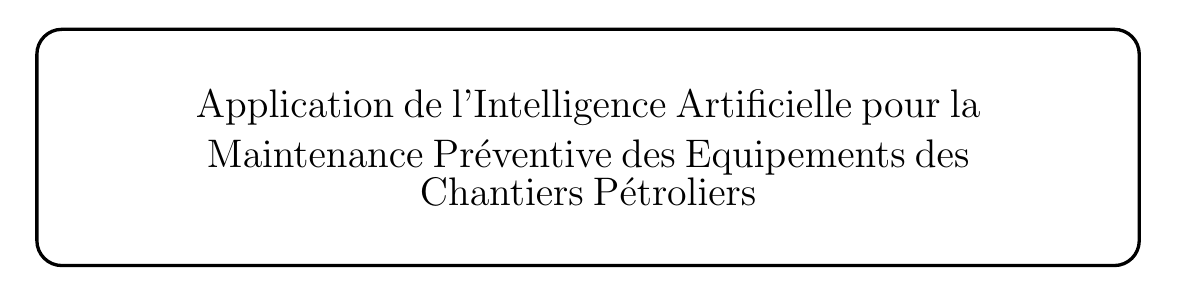
\begin{tikzpicture}
\draw [very thick, rounded corners=9pt] (-7,-1.5) rectangle (7,1.5);
\node[text width=14cm, align=center] at (0,0) {\Large Application de l'Intelligence Artificielle pour la \\Maintenance Préventive des Equipements des\\Chantiers Pétroliers};
\end{tikzpicture}

\end{center}

Devant le jury:

HALIMI Djamel\hspace{2cm} Docteur\hspace{2cm} UMBB\hspace{2cm} Encadreur

\vfill

\begin{center}
	Boumerdès : 2020
\end{center}
